\section{Make-a-Video}
\label{sec:make_a_video}


Make-a-Video \cite{make_a_video} (2022) by Meta AI is a T2V model that extends T2I capabilities to video generation using a spatiotemporally factorized diffusion model. Unlike many approaches, it doesn't require paired text-video data, enabling unsupervised training on large video datasets.

The model employs spatial and temporal SR strategies to generate high-resolution, high-frame-rate videos from text prompts. It also leverages image priors to simplify the complex task of video modeling. However, it cannot learn video-specific associations (e.g., directional hand movement) due to its reliance on unlabeled video data.

The model has 3 main stages:

\begin{itemize}
    \item Training a T2I model on text-image pairs (based on DALL-E 2 \cite{dalle_2} by OpenAI) (section \ref{sec:dalle_2}).
    \item Adapting to T2V by adding 3D convolutions and temporal attention layers to the U-Net.
    \item Unsupervised T2V training on video data, bypassing the need for paired text-video datasets.
\end{itemize}








\subsection{Architecture \& Method}

\begin{figure}
    \centering
    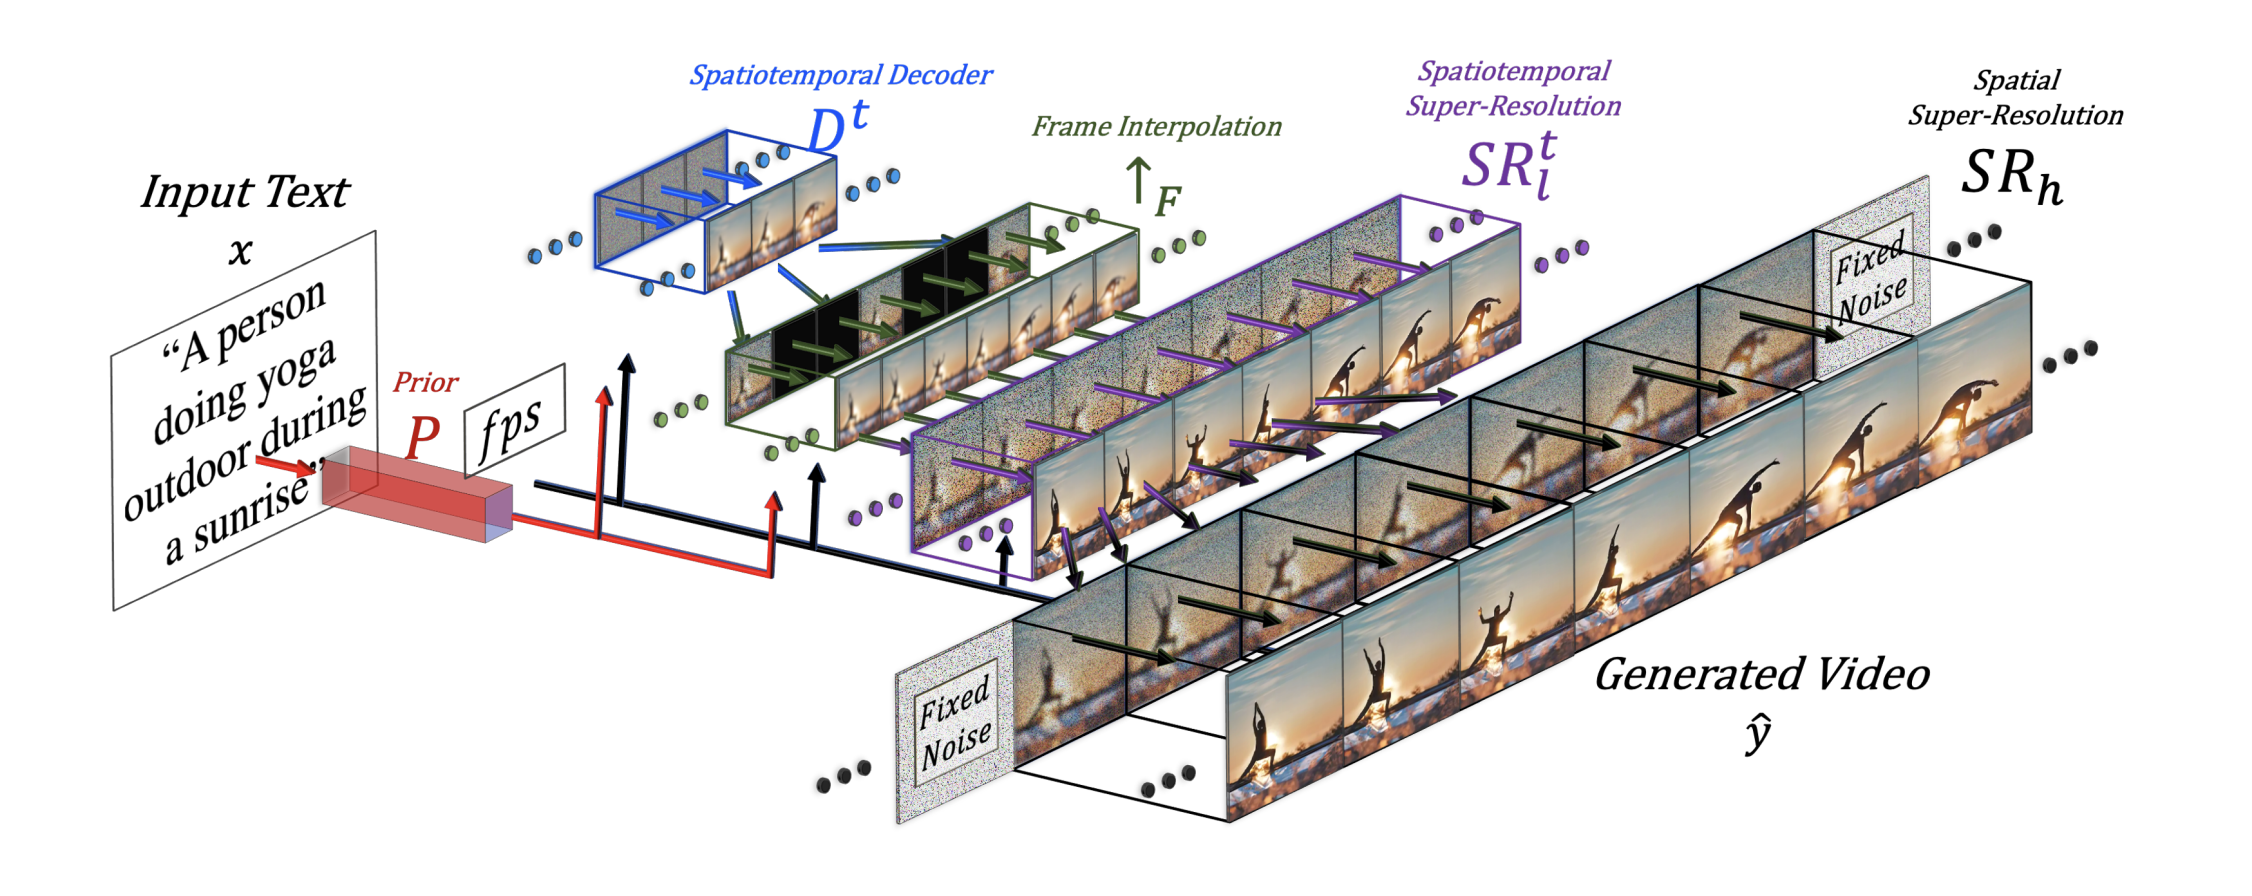
\includegraphics[width=0.7\textwidth]{images/make_a_video/overview.png}
    \caption{Make-a-Video model architecture overview \cite{make_a_video}.}
    \label{fig:make_a_video_overview}
\end{figure}

In figure \ref{fig:make_a_video_overview}:

\begin{itemize}
    \item The T2I model doesn't have "fps" input, the decoder generates only a single frame, there are interpolation networks, there are two spatial SR networks and no spatio-temporal SR network.
    \item The T2V input is a text prompt $x$ and "fps" (frames per second).
    \item It's not shown in the figure (omitted), but the input text $x$ is converted to \textbf{BPE encoding} $\hat{x}$ and given as an input to the prior $\textcolor{Maroon}{P}$ network (explained below). However, it's used in equation \ref{eq:make_a_video_inference}.
    \item The \textbf{CLIP text encoder} $C_x$ (not shown in the figure) is used to translate the text prompt $x$ into text embeddings $x_e$, which are fed to the prior network $\textcolor{Maroon}{P}$.
    \item The \textbf{image embedding prior} $\textcolor{Maroon}{P}$ translates these text embeddings $x_e$ into image embeddings $y_e$.
    \item The \textbf{spatio-temporal decoder $\textcolor{blue}{D^t}$} generates 16 $64\times 64$ frames, conditioned on these image embeddings $y_e$.
    \item These 16 images are interpolated into higher fps by the \textbf{frame interpolation model $\textcolor{OliveGreen}{\uparrow_F}$}, through masked interpolation prediction.
    \item Then these frames are increased in spatial resolution to $256\times 256$ by the \textbf{spatiotemporal super-resolution model $\textcolor{Plum}{SR_l^t}$}.
    \item And increased again to resolution $768\times 768$ by \textbf{spatial super-resolution model $SR_h$}. 
    \item The final output is high-spatiotemporal-resolution video $\hat{y}$.
\end{itemize}

The formal mathematical formulation of the Make-a-Video is:

\begin{equation}
    \hat{y_t} = \text{SR}_h \circ \textcolor{Plum}{\text{SR}_l^t} \circ \textcolor{OliveGreen}{\uparrow_F} \circ \textcolor{blue}{D^t} \circ \textcolor{Maroon}{P} \circ \left( \hat{x}, C_x (x) \right)
    \label{eq:make_a_video_inference}
\end{equation}







\subsection{The T2I model}


The T2I model in Make-a-Video builds on OpenAI's unCLIP model (DALL-E 2, see section \ref{sec:dalle_2}). The T2I model is trained first, and then factorized into a T2V model to extend spatial knowledge to video (explained in section \ref{sec:make_a_video_expanding_t2i_to_video}). After inference (equation \ref{eq:make_a_video_inference}), images are downsampled to $512\times 512$ using bicubic interpolation for cleaner aesthetics.







\subsubsection{DALL-E 2}
\label{sec:dalle_2}

DALL-E 2 by OpenAI \cite{dalle_2} is a diffusion-based T2I model, which leverages contrastive models like CLIP for image generation. They proposed a two-stage model: 

\begin{itemize}
    \item a prior network $P(z_i | y)$ that generates CLIP image embeddings $z_i$ conditioned on captions
    \item and a diffusion based decoder $P(x | z_i, y)$ that generates images $x$ conditioned on these image embeddings $z_i$, and optionally the captions $y$.
\end{itemize}

\begin{figure}
    \centering
    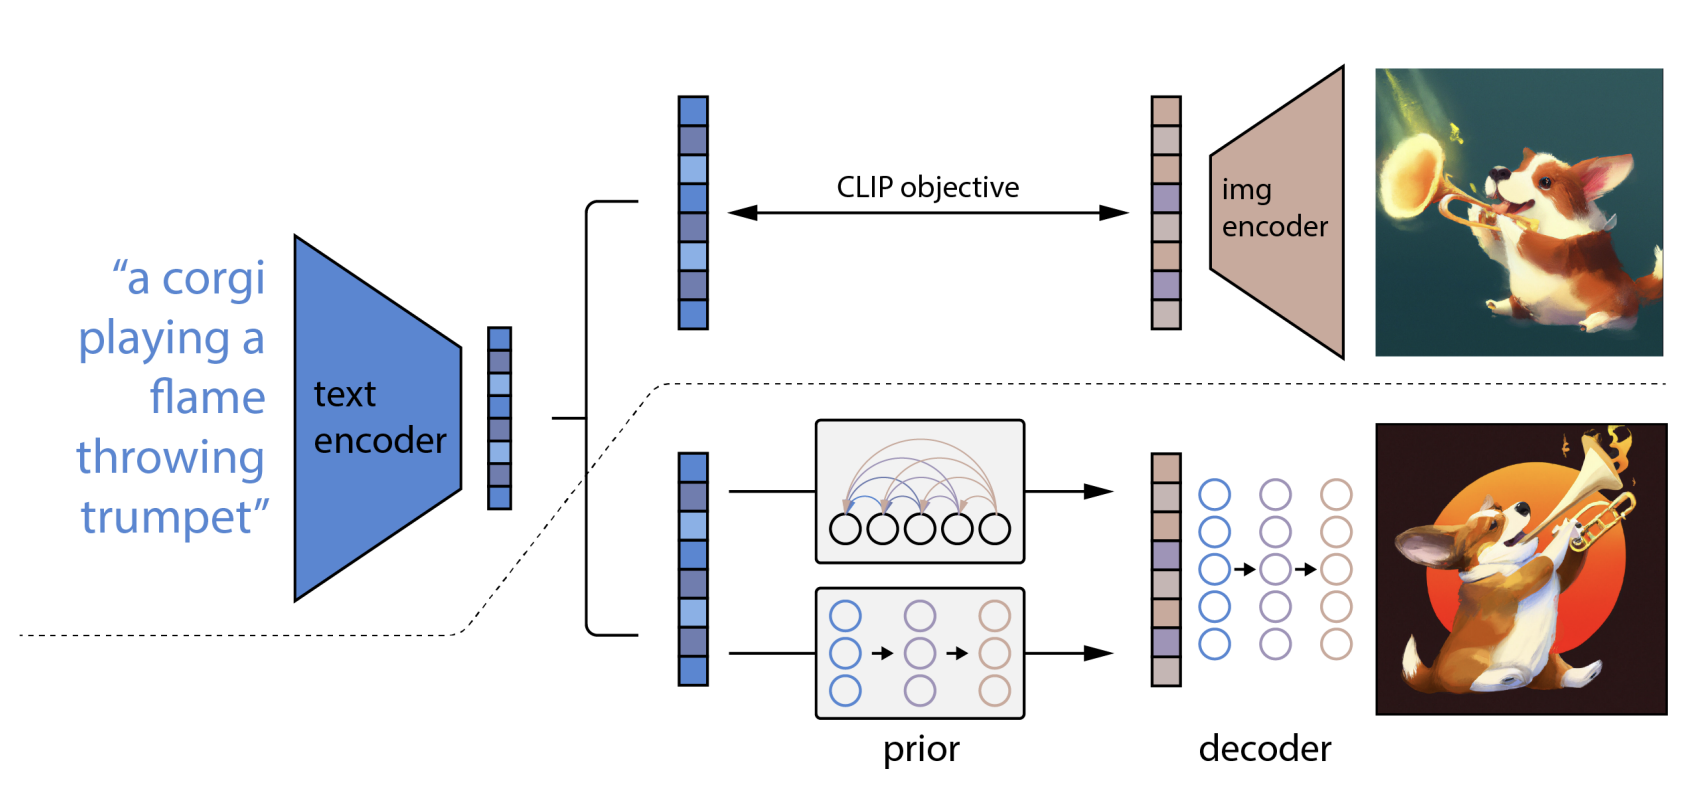
\includegraphics[width=0.6\textwidth]{images/make_a_video/dalle_2.png}
    \caption{High level overview of unCLIP (DALL-E 2) \cite{dalle_2}. \textit{Top}: the contrastive training objective of DALL-E 2; \textit{Bottom}: the inference process \cite{dalle_2}.}
    \label{fig:make_a_video_dalle2_overview}
\end{figure}

In figure \ref{fig:make_a_video_dalle2_overview} the prior model takes the CLIP text embeddings $z_t$ (the blue vector in the figure) and generates image embeddings $z_i$. Then the decoder (which acts as inverted CLIP encoder) takes in image embeddings $z_i$ (the brown vector in the figure) and generates the final image:

\begin{itemize}
    \item \textbf{Input}: the training dataset are pairs $(x,y)$ of images $x$ and captions $y$.
    \item \textbf{Output}: a single generated image $x$ given a caption $y$.
    \item \textbf{CLIP encoder} is applied to the text $x$ and caption $y$ to get text and image embeddings $z_i$ and $z_t$ respectively.
    \item \textbf{Training objective}: the text embedding $z_t$ should match the CLIP objective to the image embeddings $z_i$.
    \item \textbf{The prior network} maps the text embeddings $z_t$ to a \textit{distribution} of possible image embedding vectors $z_i$. In their experiments, they tried two different prior networks:
        \begin{itemize}
            \item \textbf{Autoregressive prior}: the image embedding $z_i$ is converted to a sequence of discrete codes and predicted autoregressively conditioned on the caption $y$. This network is based on the transformer architecture.
            \item \textbf{Diffusion based prior} where the latent vector $z_i$ is modeled using Gaussian diffusion model conditioned on caption $y$. The diffusion model is a decoder-only transformer, instead of a standard U-Net, similar to Diffusion Transformer \cite{diffusion_transformer} (appendix \ref{appendix:diffusion_transformer}).
        \end{itemize}
    \item \textbf{Decoder network}: given image embeddings $z_i$, the unCLIP network generates the final image. 
    \item \textbf{Classifier-free guidance}: they also used CFG to improve the quality of the generated images and match the captions.
    \item \textbf{Sampling in DALL-E}: first we sample $z_i$ using the prior network, and then we sample $x$ using the decoder (given $z_i$).
    \item \textbf{Super-resolution}: they also trained two SR diffusion-based networks to upsample the final generated image from $64\times 64$ to $256\times 256$ and finally to $1024\times 1024$.
    \item \textbf{x-prediction}: In the prior network, instead of predicting the noise directly ($\epsilon$-prediction), they chose to predict the unnoised $z_i$ directly (called $x$-prediction).
\end{itemize}








\subsection{Expanding the T2I model to video domain}
\label{sec:make_a_video_expanding_t2i_to_video}

The researchers modify the T2I model and transfer the image knowledge to video domain by expanding the 2D conditional network into the temporal dimension.

In short, they support the temporal dimension by adding 3D convolutions temporal attention layers in the U-Net backbone of the T2I diffusion model. The fully-connected layers doesn't need factorization since they are agnostic to structured spatial and temporal information.





\subsubsection{Spatiotemporal layers}


The spatiotemporal decoder $\textcolor{blue}{D^t}$ generates 16 RGB frames at $64\times 64$ resolution instead of a single frame. The frame interpolation network $\textcolor{OliveGreen}{\uparrow_F}$ increases the FPS by interpolating these frames (figure \ref{fig:make_a_video_overview}).

\textbf{Hallucination}: the super-resolution model involves hallucinating information. In order not to have flickering artifacts, the hallucination must be consistent across frames. As a result, $\text{SR}_l^t$ operates across spatial and temporal dimensions. In order to consistent detail hallucination across frames, in $\text{SR}_h$ they use the same noise initialization for each frame.

In addition, $\textcolor{red}{\mathbf{\text{SR}_l^t}}$ operates across both spatial and temporal dimensions. The spatial layers of $\text{SR}_l^t$  were modified for spatiotemporal super-resolution ($\textcolor{red}{\mathbf{\text{SR}_l^t}}$), but $\text{SR}_h$ avoids the temporal dimension due to memory and compute constraints further down the pipeline. Consistent detail hallucination in $\text{SR}_h$ is achieved by using the same noise initialization for all frames.









\subsubsection{Pseudo-3D convolutional layers}

Due to the high compute and memory demands of 3D convolutions, the researchers used pseudo-3D convolutional layers, inspired by \cite{chollet2017xception}. This approach decouples spatial and temporal processing via depthwise separable convolution layers, enabling more efficient computation. Pseudo-3D convolutions first apply 2D convolutions on the spatial axes, followed by 1D convolutions on the temporal axis, facilitating information sharing. The formulation is:

\[ 
\text{Conv}_{\text{P3D}} (h) := \text{Conv}_{\text{1D}} (
    \text{Conv}_{\text{2D}} (h) \circ T
) \circ T \]

where $h \in \mathbb{R}^{B\times C\times F\times H\times W}$ is an input tensor, where $B,\ C,\ F,\ H,\ W$ are the batch, channels, frames, height and width respectively, and $\circ T$ is the transpose operator which swaps between spatial and temporal dimensions.

\begin{figure}
    \centering
    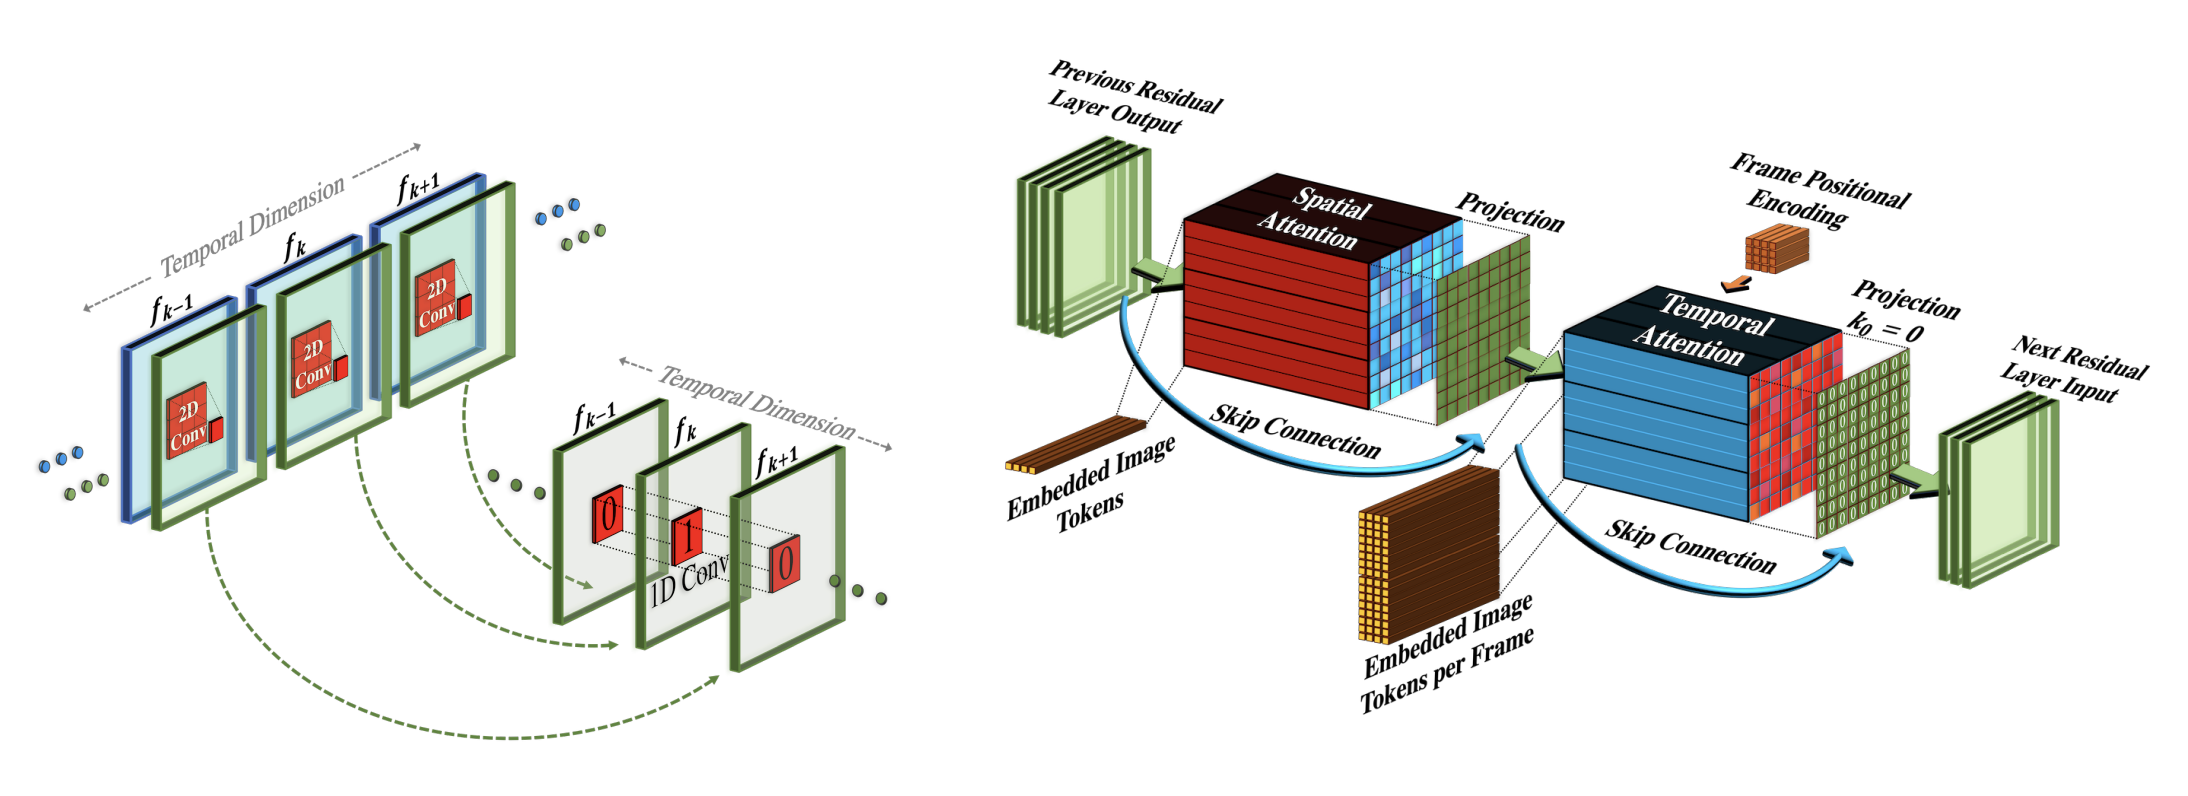
\includegraphics[width=0.8\textwidth]{images/make_a_video/pseudo_3d.png}
    \caption{Initialization of pseudo-3D convolutional (left) and temporal attention (right) layers \cite{make_a_video}.}
    \label{fig:make_a_video_pseudo_3d_conv_and_attention}
\end{figure}

In figure \ref{fig:make_a_video_pseudo_3d_conv_and_attention} we can see the pseudo-3D convolution initialization. The temporal 1D convolution layer is initialized as the identity function: it performs no transformation on the input data initially. This way the network relies on the already learned spatial features. The temporal consistency will be learned at a later stage, where the model is trained on video dataset.












\subsubsection{Pseudo-3D attention layers}

Temporal attention is computationally expensive, so the researchers used stacked pseudo-3D temporal attention layers, inspired by \cite{video_diffusion_models} (Video U-Net) and Imagen-Video \cite{imagen_video}.

Each pre-trained spatial attention layer is followed by a pseudo-3D temporal attention layer. The process involves flattening the spatial dimensions $h' \in \mathbb{R}^{B\times C\times F\times \mathbf{\textcolor{red}{HW}}}$ (\texttt{unflatten} is the inverse operation) and applying 2D and 1D attention sequentially:

\[ \text{ATTN}_{\text{P3D}} (h) = \text{unflatten} 
(\text{ATTN}_{\text{1D}} 
(\text{ATTN}_{\text{2D}} 
(\text{flatten} (h)) \circ T) \circ T) 
\]

$\text{ATTN}_\text{2D}$ is initialized from the T2I model, and $\text{ATTN}_\text{1D}$ starts as the identity function (figure \ref{fig:make_a_video_pseudo_3d_conv_and_attention}) which allows smooth spatiotemporal initialization.

They also introduce FPS conditioning, inspired by \cite{cogvideo}, by adding a $\text{fps}$ parameter which enables additional augmentation that deals with the limited volume of training videos and provides more control over the generated video at inference time.







\subsection{Frame interpolation network}

The frame interpolation network $\textcolor{OliveGreen}{\uparrow_F}$ increases number of frames by interpolation or pre/post extrapolation. In addition to RGB channels, they add the binary mask channel (0 or 1) indicating which frames masked during training. This model is conditioned on $\text{fps}$ which enable multiple temporal upsample rates at inference. For extrapolation, they can use the same strategy.






\subsection{Training}

The prior network is trained on text-image pairs and is not fine-tuned for videos.

Initially, the decoder, prior, and two super-resolution (SR) networks are trained on images. Temporal layers are then added, and the models are fine-tuned using unlabeled video data.

To train the T2I model, they used 2.3B subset of Laion-5b \cite{laion_5b} of image-text pairs.

To train the T2V model, they used:

\begin{itemize}
    \item WebVid-10M \cite{webvid_10m} text-to-video dataset - which was used to train both the decoder, the interpolation network, and the $\text{SR}_h$ networks.
    \item and a 10M subset from HD-VILA-100M \cite{hd_vila_100m} - which was used to train $\text{SR}_h$.
\end{itemize}






\subsection{Experiments}

They conducted evaluation on UCF-101 \cite{ucf_101} and MSR-VTT \cite{msr_vtt} datasets in zero-shot setting. The researchers also used DrawBench prompts from Imagen for human evaluation.




\subsubsection{Quantitative Results}

\begin{figure}[h]
    \centering
    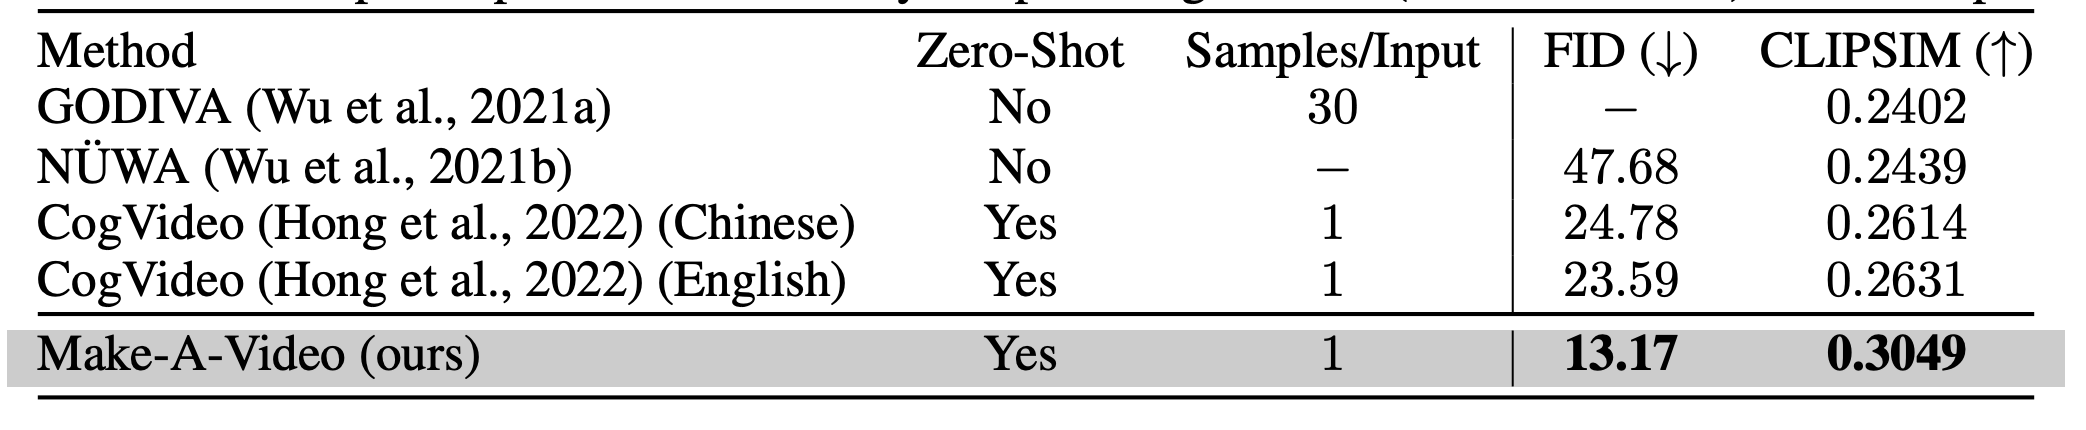
\includegraphics[width=0.7\textwidth]{images/make_a_video/zero_shot_eval.png}
    \caption{Zero-shot MSR-VTT evaluation of Make-a-Video \cite{make_a_video}.}
    \label{fig:make_a_video_zeroshot_eval}
\end{figure}

Evaluation on MSR-VTT \cite{msr_vtt} text-video dataset is shown in figure \ref{fig:make_a_video_zeroshot_eval}. Make-a-Video significantly outperforms all state-of-the-art T2V generation models in zero-shot setting in both FID and CLIP-SIM score.

\begin{figure}[h]
    \centering
    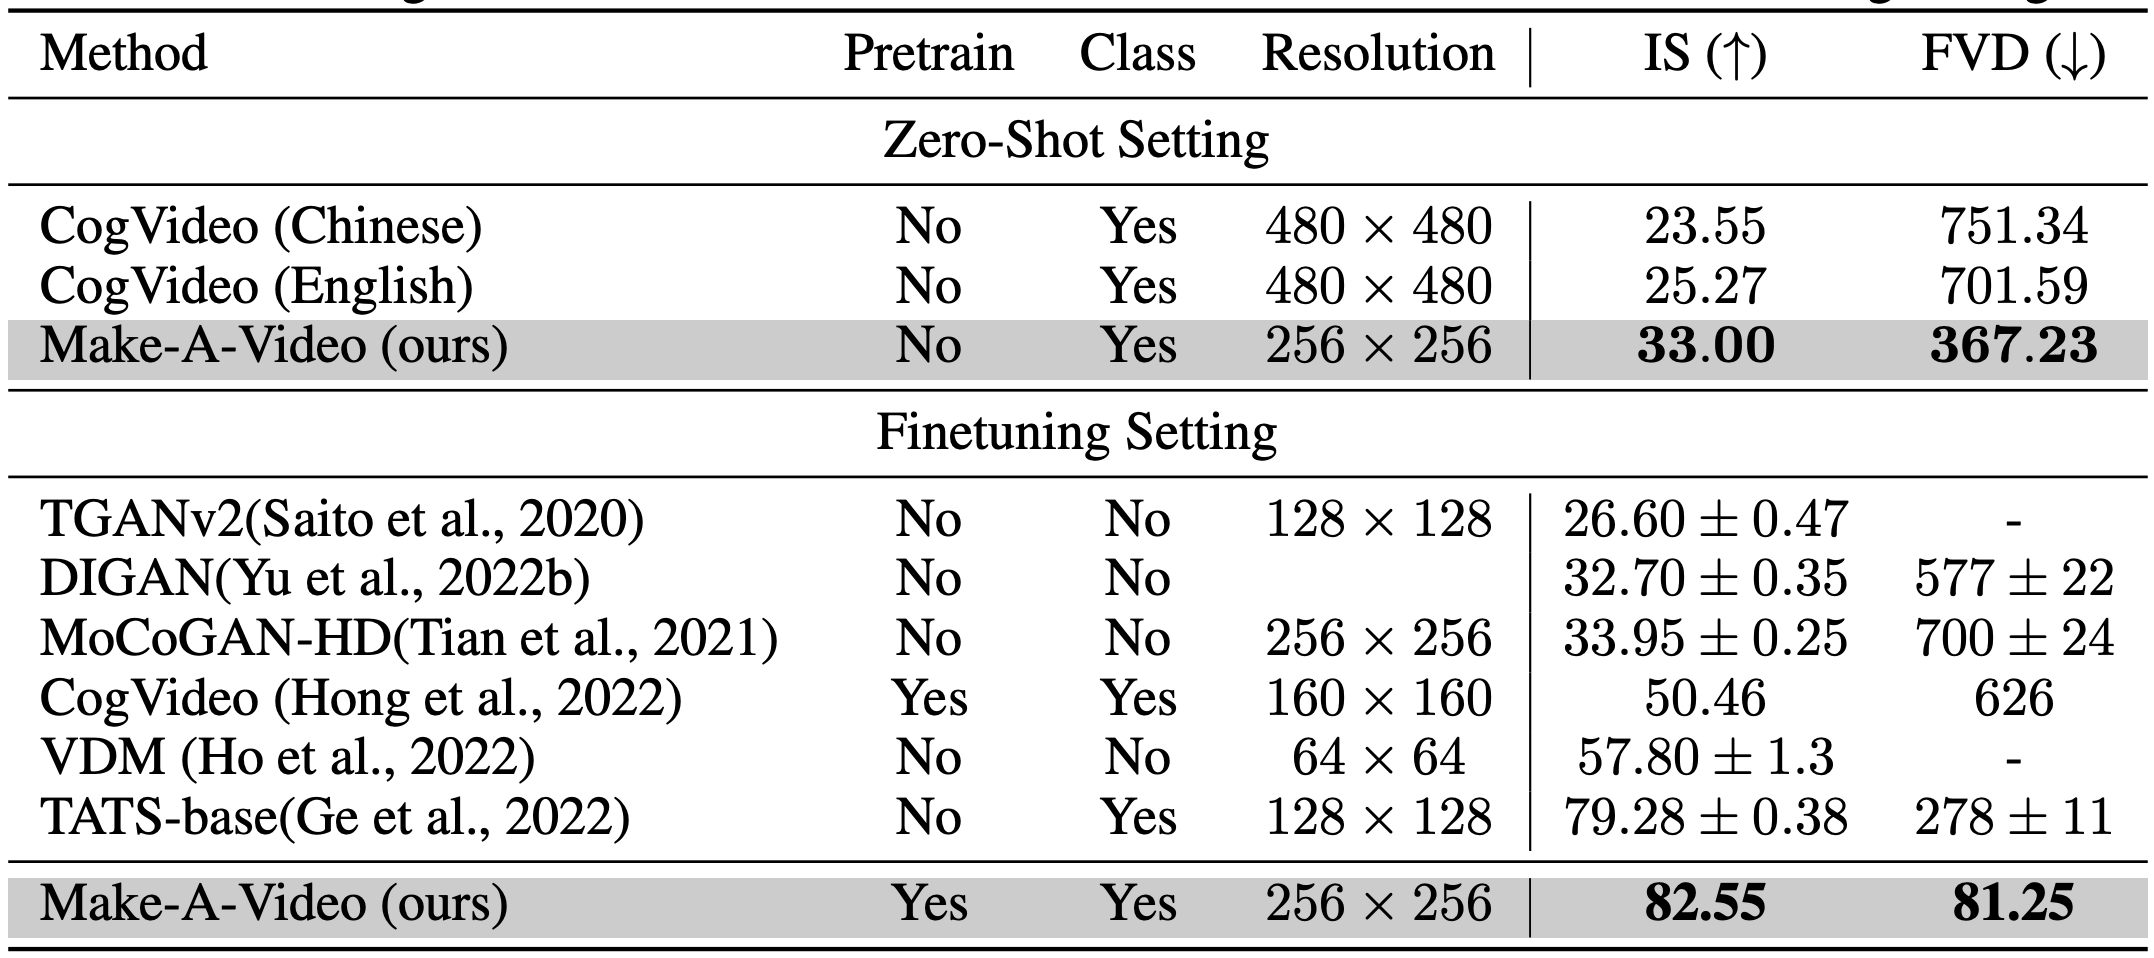
\includegraphics[width=0.7\textwidth]{images/make_a_video/ucf_101.png}
    \caption{Zero-shot and fine-tuning evaluation on UCF-101 dataset \cite{make_a_video}.}
    \label{fig:make_a_video_ucf_101}
\end{figure}

Evaluation on UCF-101 is shown in figure \ref{fig:make_a_video_ucf_101}. Make-a-video also outperforms all the other models in IS, FVD metrics.

\begin{figure}[h]
    \centering
    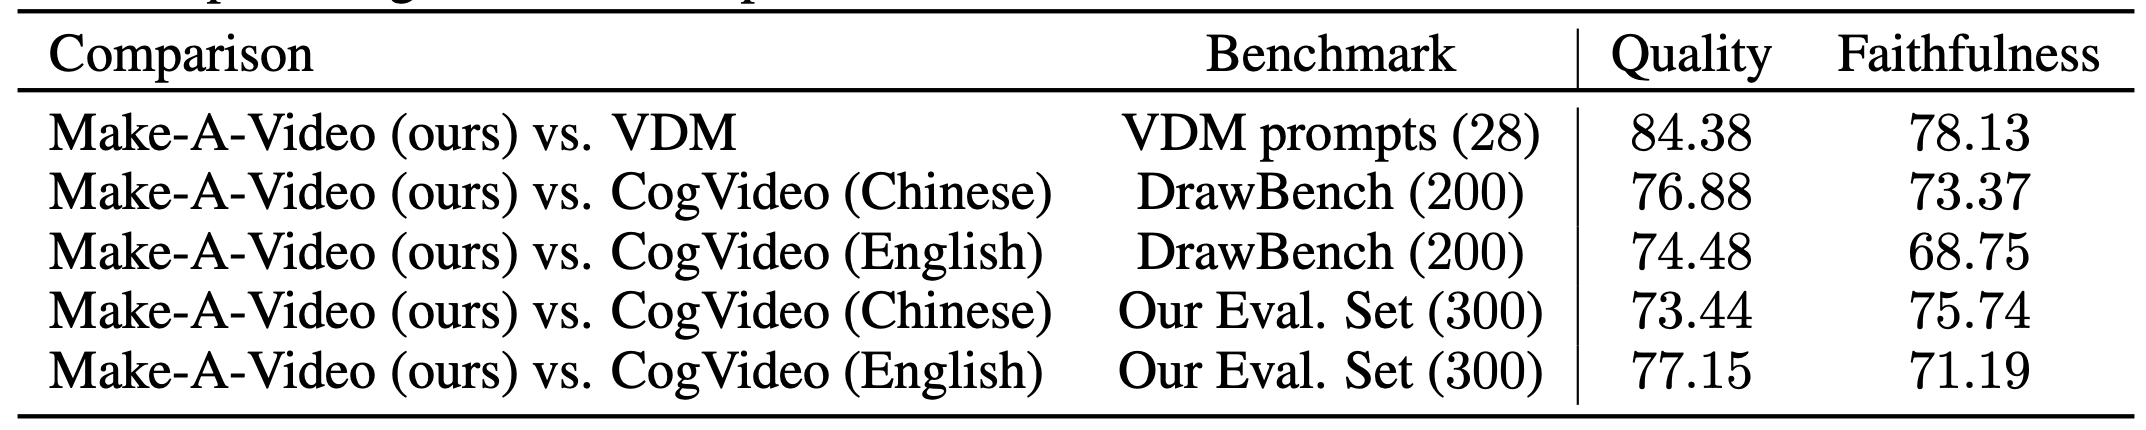
\includegraphics[width=0.7\textwidth]{images/make_a_video/eval.png}
    \caption{Make-a-Video human evaluation on DrawBench benchmark. The numbers in \texttt{()} indicate amount of videos compared in each evaluation \cite{make_a_video}.}
    \label{fig:make_a_video_human_eval}
\end{figure}

In human evaluation (shown in figure \ref{fig:make_a_video_human_eval}), they asked humans which video (out of two videos chosen randomly) is higher quality. For faithfulness, they show the text description of the video in addition to the video, and ask which video has better correspondence with the text (text-video alignment).




\subsubsection{Qualitative Results}

The qualitative results of Make-a-Video is remarkable. We see some samples in figures \ref{fig:make_a_video_examples} and \ref{fig:make_a_video_examples2}.

\begin{figure}
    \centering
    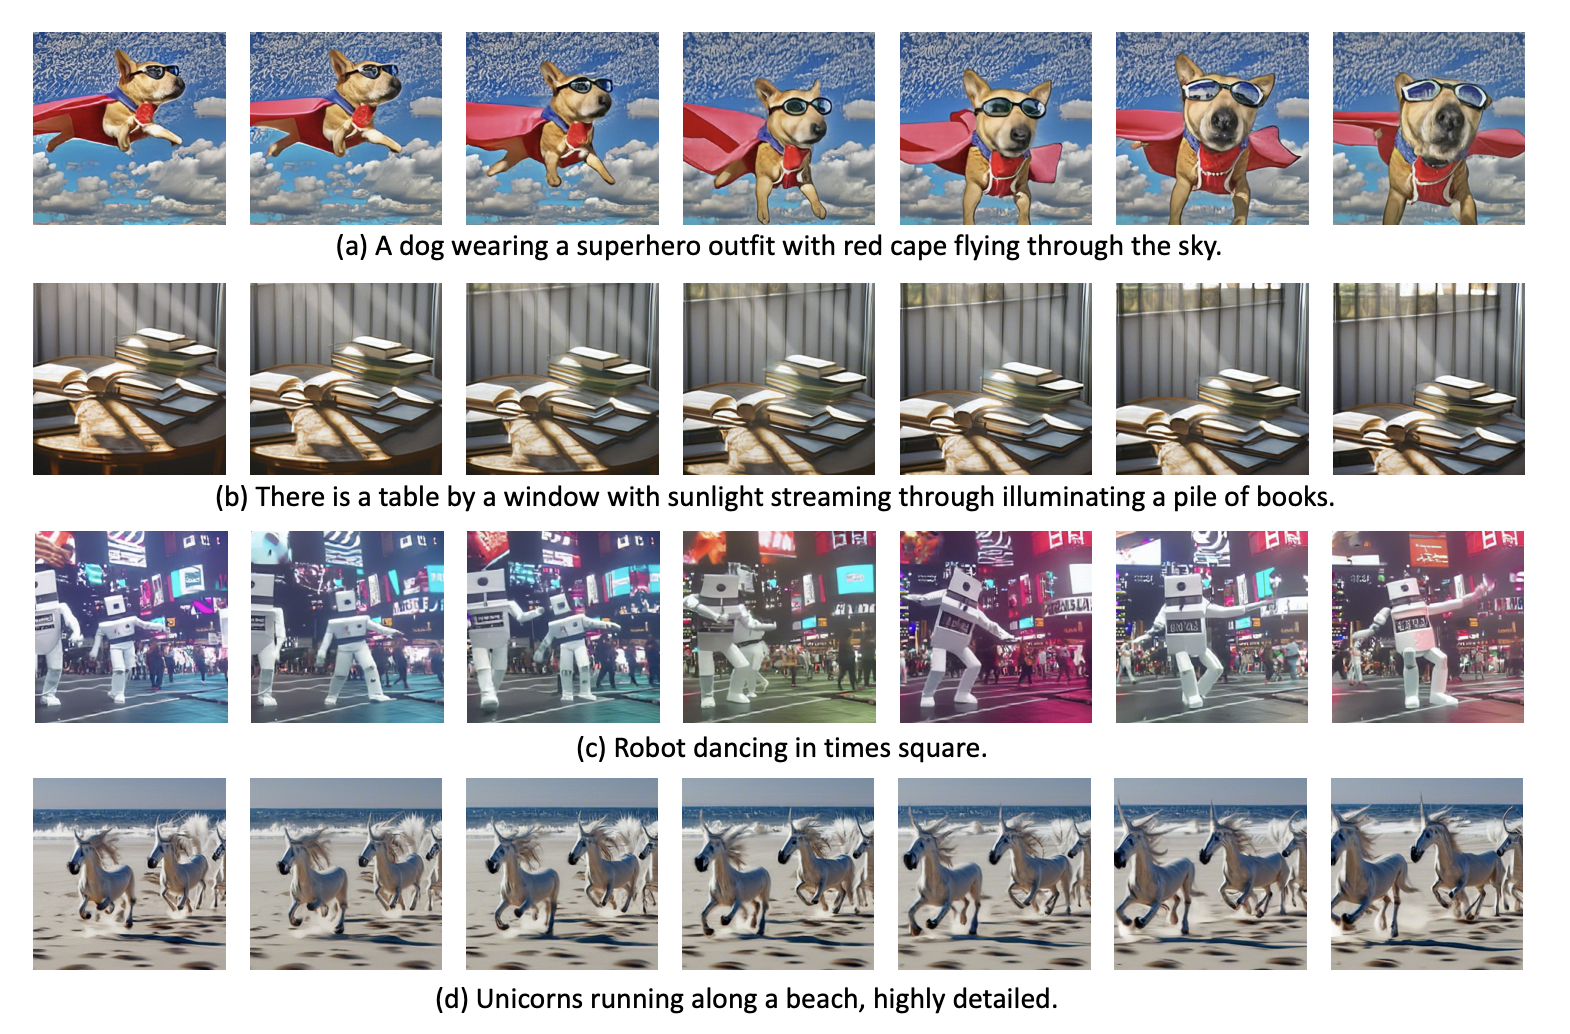
\includegraphics[width=0.7\textwidth]{images/make_a_video/examples.png}
    \caption{Examples of T2V samples of Make-a-Video \cite{make_a_video}.}
    \label{fig:make_a_video_examples}
\end{figure}

\begin{figure}
    \centering
    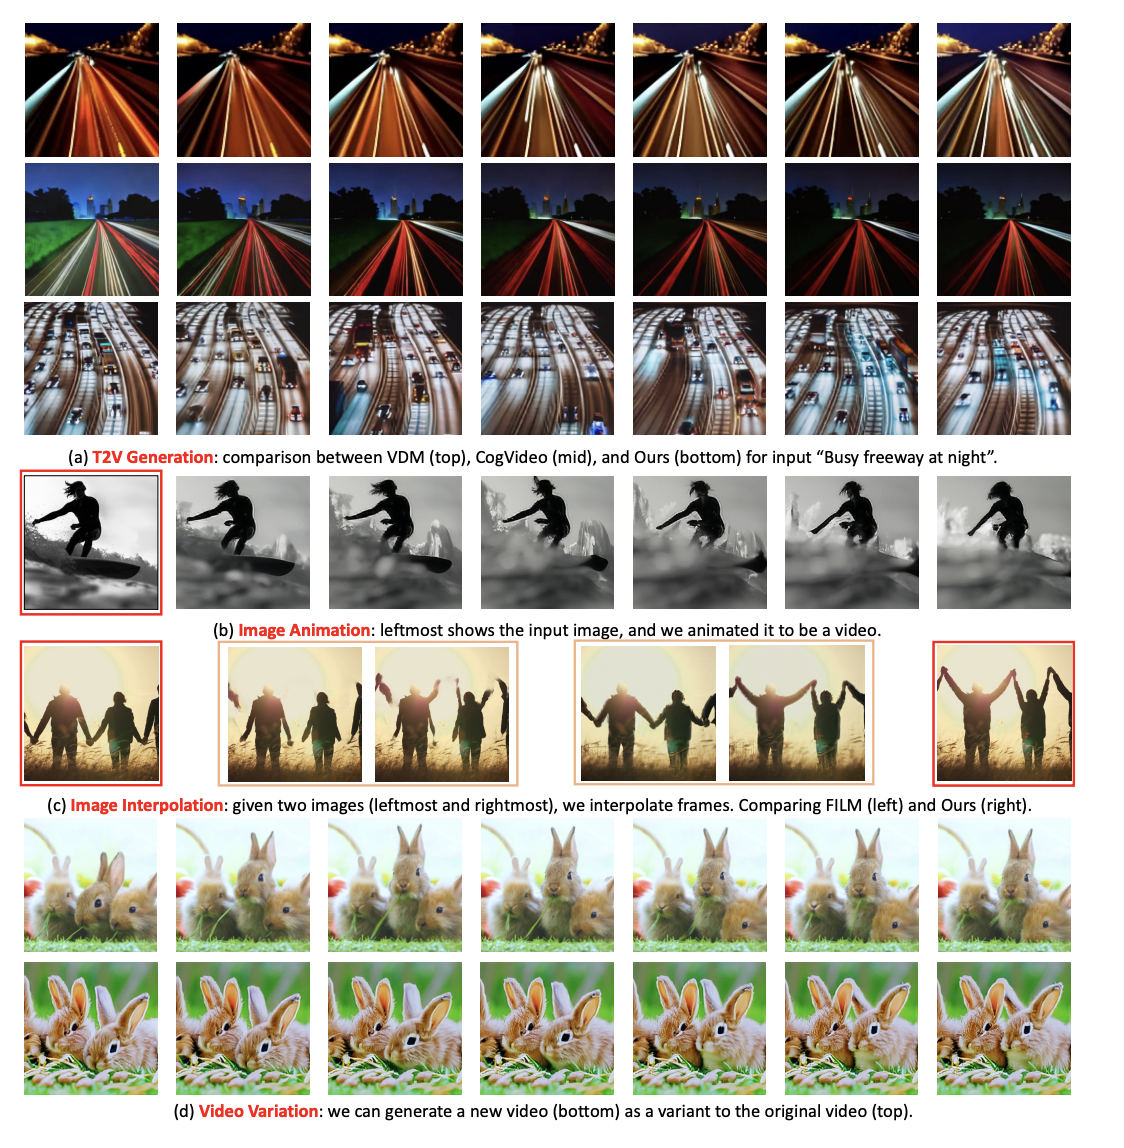
\includegraphics[width=0.7\textwidth]{images/make_a_video/examples2.png}
    \caption{Various qualitative results comparisons and applications \cite{make_a_video}.}
    \label{fig:make_a_video_examples2}
\end{figure}

In figure \ref{fig:make_a_video_examples2} (c) we see the interpolation network works better than FILM \cite{film} by Google, which is a model specifically learned to interpolate between frames.

